\documentclass{article}

% hide the (ugly) borders of links
\usepackage[hidelinks]{hyperref}

% no indentation at paragraph, use line break instead
\usepackage[parfill]{parskip}

% math package
\usepackage{amsmath}
\usepackage{amsthm}
\usepackage{amssymb}
\usepackage{mathrsfs}

\usepackage{float}

% custom headers and footers
\usepackage{fancyhdr}

% count page number
\usepackage{lastpage}

% multicolumn
\usepackage{multicol}

% customized margin
\usepackage[top=1in, bottom=1in, left=1in, right=1in]{geometry}

\usepackage{algorithm2e}

\usepackage{graphicx}
\graphicspath{ {figs/} }

% personal info
\newcommand{\id}{Person \texttt{\#}: \texttt{5009 4218}}
\newcommand{\email}{\href{mailto:jinghaos@buffalo.edu}{jinghaos@buffalo.edu}}
\newcommand{\name}{Jinghao Shi}

% cover page
\newcommand{\makecoverpage}{
\maketitle
\thispagestyle{empty}
\newpage
% for double side printing, leave backside of cover page blank
\begin{center}
  \vspace*{\fill}
  \LARGE{\textit{This page intentionally left blank.}}
  \vspace*{\fill}
\end{center}
\thispagestyle{empty}
\newpage
% reset page number counter
\setcounter{page}{1}
}

\newcommand{\problem}[1]{\textbf{Problem.}\quad #1}
\newcommand{\solution}[1]{\textbf{Solution.}\quad #1}
\newcommand{\key}[1]{\textbf{#1}\quad}

\title{\vspace{2in}
CSE596: Introduction to the Theory of Computation \\
\vspace{0.5in}
Glossary\\
\vspace{3in}
}

\author{
\name\\
\email\\
}

% header and footer
\pagestyle{fancy}
\lhead{\leftmark}
\rhead{CSE596 Glossary}
%\rhead{\name\\\email}
\cfoot{\thepage ~/ \pageref{LastPage}}
\renewcommand{\headrulewidth}{0.5pt}

\begin{document}
\makecoverpage

\section{Preliminaries}

\subsection{Words and Language}

\key{Alphabet} A finite set of symbols. $\Sigma=\{a_1, a_2,\ldots,a_k\}$.

\key{Word} A finite sequence of symbols.

\key{Language} A set of words. $L \in \Sigma^*$.

\subsection{Partial Functions}

\key {Partial Function} $f: X' \rightarrow Y, \text{where } X' \subset X$.

\key{Total Function} When $X' = X$.

\key{Converge} When $f(x)$ is defined. Noted as $f(x) \downarrow$.

\key{Diverge} When $f(x)$ is not defined. Noted as $f(x) \uparrow$.

\subsection{Propositional Logic}

\key{Satisfiable}  A formula $F$ is
satisfiable if there exists an assignment to its variables that satisfies it.

\key{Tautology} A formula is valid (or is a tautology) if every assignment to
its
variables satisfies it

\key{Conjunction} $A_1 \land A_2 \land \cdots \land A_n$

\key{Disjunction} $A_1 \lor A_2 \lor \cdots \lor A_n$

\key{Clause} Disjunction of literals.

\key{Conjunctive Normal Form (CNF)} Conjunction of clauses.

\subsection{cardinality}

\key{Same Cardinality} $card(A) = card(B) \text{ iff. } \exists f: A \rightarrow
B$ is a bijection.

\key{Countable} A set $A$ is countable if $card(A) = card(N)$
or $A$ is finite.

\key{Countable Infinite} $card(A) = card(N)$.

\key{Enumerable} A set is enumerable if it is the empty set or there is a
function $f : N \rightarrow_{onto} A$, i.e., $A = range(f) = \{a_0, a_1, \ldots\}$

\key{Enumerable $\Rightarrow$ Countable} Define $h$ as follows:
\begin{align*}
  h(0) &= f(0) \\
  h(n+1) &= f(min\{x|f(x) \notin \{h(0), h(1),\ldots, h(n)\}\})
\end{align*}
\begin{itemize}
  \item $h$ is one-to-one since $h(n+1) \notin \{h(0), h(1),\ldots,h(n)\}$. \\
  \item $range(h) \subseteq range(f) = S$. \\
  \item $f(0)=h(0)$, suppose by induction that $f(n) \in \{h(0),h(1),\ldots,h(n)\}$ and $f(n+1) \notin
    \{h(0), h(1),\ldots,h(n)\}$, then $n+1 = min\{x|f(x) \notin
    \{h(0),h(1),\ldots,h(n)\}\}$, so $h(n+1)=f(n+1)$. So $\forall n, f(n) \in \{h(0),
    h(1),\ldots,h(n)\}$, $S=range(f) \subseteq range(h)$.\\
\end{itemize}
Thus $S=range(f) = range(h)$, $h:N\rightarrow_{1-1}S$, $card(N)=card(S)$

\key{Theorem 1.3.} A set $A$ is countable if and only if $card(A) \le
\mathbf{\aleph}_0$.
\begin{align*}
& card(A) \le \aleph_0 \\
\Rightarrow & \exists f:A \rightarrow_{1-1} N \\
\Rightarrow & f[A] \text{ doesn't have a largest number (otherwise, } A \text{ is
finite.)}\\
\Rightarrow & a_0 = min\{f[A]\}, a_{n+1}=min\{f[A]-\{f(0),f(1),\ldots,f(n)\}\}
\\
\Rightarrow & A \text{ is enumerable.} \\
\Rightarrow & A \text{ is countable.}
\end{align*}

\key{Theorem 1.4.} The set of all functions from $N$ to $N$ is not countable.\\
Let $A=\{f|f:N \rightarrow N\}$, suppose for contradiction that $A$ is countable,
then $A=\{f_1,f_2,\ldots\}$, define $g(x)=f_x(x)+1$ and $g = f_k$ for some $k$,
but $g(k)=f_k(k)+1 \neq f_k(k)$.

\key{Theorem 1.5.} $\mathscr{P}(N)$ has cardinality greater than $\aleph_0$.\\
Let $A=\mathscr{P}(N) = \{S|S \subseteq N\}$ is power set of $N$. Suppose for
contradiction that $A$ is enumerable, then $A=\{S_0,S_1,\ldots\}$, define
$T=\{k|k\notin S_k\}$ and $T \in A$. However, $\forall k\; T \neq S_k$ since $k
\in T \Leftrightarrow k \notin S_k$.

\subsection{Misc}

\key{onto/surjection} $f: A \rightarrow_{onto} B \text{ iff. } \forall b \in B, \exists a
\in A \text{ s.t. } f(a) = b$

\key{one-to-one/injection}  $f: A \rightarrow_{1-1} B \text{ iff. } f(a)=f(b)
\Rightarrow a=b$

\key{bijection} Both one-to-one and onto.



\section{Turing Machine and RAM}

\subsection{Turing Machine}

\key{Turing Machine} $M=\langle
Q,\Sigma,\Gamma,\delta,q_0,B,q_{accept},q_{reject}\rangle$

\key{TM-acceptable} A language $L, L \subseteq \Sigma^*$, is
Turing-machine-acceptable if there is a Turing machine
that accepts L.

\key{TM-decidable} A language L is Turing-machine-decidable if L is accepted by
some
Turing machine that halts on every input.

\key{$L(M)$} $L(M)=\{w \in \Sigma^* | M \text{ accepts } w \}$.

\key{$M$ computes $\phi$} $M$ eventually enter an accepting configuration of
$\phi(w_1,\ldots,w_n)q_{accept}$ iff.
$\phi(w_1,\ldots,w_n)\downarrow$.

\key{Partial Computable} A partial function $\phi$ is partial computable if there
is some Turing machine
that computes it.

\key{Total Computable} $\phi(w_1,\ldots,w_n)\downarrow$ for all
$w_1,\ldots,w_n$. If $M$ computes a total computable function, $L(M)=\Sigma^*$.

\key{Theorem 2.2.} A language $L$ is decidable if and only if both $L$ and
$\bar{L}$ are acceptable.\\
Parallel simulation.

\key{RAM}
\begin{table}[H]
  \begin{tabular}{lll}
    $1_j$ & $X\;\mathbf{add}_j\;Y$ & append $a_j$ to $Y$\\
    $2$ & $X\;\mathbf{del}\;Y$ & delete right most symbol of $Y$\\
    $3$ & $X\;\mathbf{clr}\;Y$ & $Y \rightarrow \lambda$\\
    $4$ & $X\;Y\leftarrow Z$ & $Y=Z$\\
    $5$ & $X\;\mathbf{jmp}\;Y$\\
    $6_j$ & $X\;Y\;\mathbf{jmp}_j\;X'$\\
    $7$ & $X\;\mathbf{continue}$
  \end{tabular}
\end{table}



\section{Undecidability}

\subsection{Decision Problems}

\subsection{Undecidable Problems}

\key{Characteristic Function} 
$f_{S}(x) = \begin{cases}
  0 & \text{if } x \in S \\ 
  1 & \text{if } x \notin S
\end{cases}$

\key{Proposition 3.1.} A set $S$ is decidable if and only if its characteristic
function is computable.

\key{$w_M$} The word that encodes $M$.

\key{G\"odel Number $e$} The code for a Turing machine $M$.

\key{$\phi_e=\lambda x.U(e,x).$} $\phi_e$ is the partial function of one
argument that is computed by $M_e$.

\key{Theorem 3.1.} The Program Termination problem (Example 3.2) is undecidable.
There is no algorithm to determine whether an arbitrary partial computable
function is total. Thus, there is no algorithm to determine whether a Turing
machine
halts on every input.\\
Define
\begin{align*}
  \text{TEST}(i) = 
  \begin{cases}
    \text{``yes''} & \text{ if } \phi_i \text{ halts on every input.} \\
    \text{``no''} & \text{ otherwise}
  \end{cases}
\end{align*}

\begin{align*}
  \delta(k) =
  \begin{cases}
    \phi_k(k)+1 & \text{ if TEST(i)="yes"} \\
    0 & \text{ if TEST(k)="no"}
  \end{cases}
\end{align*}
Thus $\delta$ is total computable. Let $\delta=\phi_e$, then TEST(e) is ``yes''.
$\delta(e)=\phi_e(e)+1 \neq \phi_e(e)$.

\subsection{Pairing Functions}
\key{Paring function} Computable one-to-one mapping $<,>:N \times N \rightarrow
N$, whose inverse $\tau_1(<x,y>)=x$ and $\tau_2(<x,y>)=y$ are also computable.\\
Example, $<x,y>=\frac{1}{2}(x^2+2xy+y^2+3x+1)$.


\subsection{Computably Enumerable Sets}
\key{Computable enumerable (c.e.)} A set $S$ is c.e. if $S=\emptyset$ or
$S=range(f)$ in which $f$ is a total computable function.

\key{index set} Let $\mathscr{C}$ be any set of partial computable functions,
then $P(\mathscr{C})=\{e|\phi_e \in \mathscr{C}\}$ is called index set.

\key{Effectively enumerable} A collection of Turing machines is effectively
enumerable if the corresponding set of G\"odel numbers is c.e.

\key{Homework 3.3} $A=\{(e,j)|L(M_e) = L(M_j)\}$ is not decidable.\\
Suppose by contradiction that $A$ is decidable, let $L(M_j)=\Sigma^*$, then
$\{e|L(M_e)=\Sigma^*\}=\{e|\phi_e \text{ is total computable}\}$ is decidable,
this contradicts \textbf{Theorem 3.1}.

\key{Theorem 3.2.} $\{e | \phi_e is \text{ total computable}\}$ is not
computably enumerable.\\
Let $S=\{e|\phi_e \text{ is total computable}\}$ and suppose for contradiction
that $S$ is c.e., then $S=range(g)$ for some total computable function $g$.
Define $U_S(e,x)=\phi_{g(e)}(x)$ and $h(x)=U_S(x,x)+1$, so $\exists k \in S
\text{ s.t. } h=\phi_k$ and $\exists e \text{ s.t. } k=g(e)$.
Finally,
\begin{align*}
  \phi_k(e)&=h(e)\\
  &=U_S(e,e)+1 \\
  &=\phi_{g(e)}(e)+1\\
  &=\phi_k(e)+1
\end{align*}

\key{Theorem 3.3.} A set $S$ is computably enumerable if and only if there is a
decidable
relation $R(x, y)$ such that
\begin{align*}
x \in S \Leftrightarrow \exists y R(x, y).
\end{align*}

\key{Theorem 3.4.} A set $S$ is computably enumerable if and only if it is
Turing-machine-
acceptable.

\key{Corollary 3.1.} A set $S$ is decidable if and only if $S$ and $\bar{S}$ are both
computably
enumerable.

\key{Corollary 3.2.} A set $S$ is computably enumerable if and only if $S$ is the
domain of
some partial computable function.

\key{Homework 3.4} Prove that an infinite set is decidable if and only if it can
be
enumerated in increasing order by a one-to-one total computable function.

\key{Homework 3.6} Prove that every infinite c.e. set contains an infinite
decidable subset.
\begin{align*}
  h(0) &= f(0)\\
  h(n+1) &= f(min\{x|f(x) \notin \{h(0), h(1),\ldots, h(n)\}\})
\end{align*}

\key{$W_e=dom(\phi_e)$}

\subsection{Halting Problem, Reductions, and Complete Sets}

\key{Diagonal Set} $K=\{x|\phi_x(x)\downarrow\}=\{x|U(x,x)\downarrow\}$=\{TM
that accepts its own code.\}. Since $\lambda x.U(x,x)$ is partial computable,
$K$ is c.e.

\key{Theorem 3.5.} $K$ is not decidable. In particular, $\overline{K}$ is not
c.e.\\
Suppose $\bar{K} = W_e = dom(\phi_e)$, then $e \in \bar{K} \Leftrightarrow
\phi_e(e)\downarrow \Leftrightarrow e \in K$.

\key{Many-one reducible} $A \le_m B$ if there is a total computable function
s.t. $x \in A \Leftrightarrow f(x) \in B$

\key{Lemma 3.2.} 1. If $A \le_m B$ and $B$ is c.e., then $A$ is c.e.\\
2. If $A \le_m B$ and $B$ is decidable, then $A$ is decidable.

\key{Theorem 3.6.} The Halting problem is undecidable. Specifically, the set
$L_U=\{(e,w)|M_e \text{ accepts } w\}$ is not decidable.\\
$x \in K \Leftrightarrow (x,x) \in L_U$, $x \mapsto (x,x)$ is total, so $K \le_m
L_U$.

\subsubsection{Complete Problems}
\key{Many-one complete} $L$ is many-one complete if
\begin{enumerate}
  \item $L$ is c.e.
  \item For every c.e. set $A$, $A \le_m L$
\end{enumerate}

\key{Homework 3.8} Show that $K$ is a many-one complete set. Note that it suffices
to show that $L_U \le_m K$.\\
Need to show $(e,w) \in L_U \Leftrightarrow f((e,w)) \in K$ for some total
computable function $f$. Define $f((e,w)) = e'$ where $M_e'$ is defined as
follows.\\
\begin{algorithm}[H]
  on input x\;
  \uIf{$M_e$ accepts $w$}{
    ACCEPT\;
  }
  \Else{
    REJECT\;
  }
\end{algorithm}
Then we have
\begin{align*}
  (e,w) \in L_U & \Leftrightarrow L(M_e')=\Sigma^*\\
  & \Leftrightarrow e' \in L(M_e')\\
  & \Leftrightarrow e' \in K
\end{align*}

Decidable sets are a proper subclass of the set of all c.e. sets

\subsection{S-m-n Theorem}

\key{Corollary 3.3.} For every partial computable function $\lambda x.\Psi(e,x)$,
there is a total computable function $f$ so that $\phi_{f(e)}(x) = \Psi(e,x).$

\key{Theorem 3.9.} There is a total computable function $f$ such that
$range \phi_{f(e)} = dom \phi_e$.\\
Define 
\begin{align*}
  \Psi(e,x)=
  \begin{cases}
    x & \text{ if } x \in dom\phi_e\\
    \uparrow & \text{ otherwise.}
  \end{cases}
\end{align*}
So $range(\lambda x.\Psi(e,x)) = dom\phi_e$, and $\phi_{f(e)}=\Psi(e,x)$, so
$range(\phi_{f(e)}) = dom\phi_e$.

\key{Homework 3.9} Prove that there is a total computable function $g$ such that
$dom\phi_{g(e)} = range\phi_e$.\\
Define
\begin{align*}
  \Psi(e,x)=
  \begin{cases}
    1 & \text{ if } x \in range\phi_e\\
    \uparrow & \text{ otherwise.}
  \end{cases}
\end{align*}
So $range(\Psi(e,x)) = range(\phi_{g(e)}(x) = range(\phi_e)$

\subsection{Recursion Theorem}

\key{Theorem 3.10.} For every total computable function $f$ there is a number
$n$
such that $\phi_n = \phi_{f(n)}$. A number $n$ with this property is called a
fixed point of $f$ .

\key{Corollary 3.5.} There is a number (i.e., program) $n$ such that $\phi_n$ is the
constant function with output $n$.\\
Define $\Psi(e,x)=e$, then $\Psi(e,x)=\phi_{f(e)}(x)=\phi_e(x) = e$.

\key{$W_n=\{n\}$} Define
\begin{align*}
  \Psi(e,x)=
  \begin{cases}
    e & \text{ if } x = e \\
    \uparrow & \text{ otherwise}
  \end{cases}
\end{align*}
$\Psi(e,x)=\phi_{f(e)}(x)=\phi_e(x)$, $dom\phi_e = \{e\}$

\key{$W_n=\{n^2\}$} Define
\begin{align*}
  \Psi(e,x)=
  \begin{cases}
    e & \text{ if } x = e^2 \\
    \uparrow & \text{ otherwise}
  \end{cases}
\end{align*}
$\Psi(e,x)=\phi_{f(e)}(x)=\phi_e(x)$, $dom\phi_e = \{e^2\}$

\key{Homework 3.11} Show that there is no algorithm that given as input a Turing 
machine $M$, where $M$ defines a partial function of one variable, outputs
a Turing machine $M'$ such that $M'$ defines a different partial function of one
variable.\\
Suppose for contradiction that such $\exists f \forall n \phi_n \ne
\phi_{f(n)}$, and $f$ is total.

\key{Theorem 3.11.} For every partial computable function $\Psi(e, x)$, there is a
value $e_0$ such that $\Psi(e_0,x) = \phi_{e_0}(x)$.

Observe that there is a standard pattern to the proof of these results. First,
we use the $s-m-n$ theorem or its corollary to obtain a total computable
function $f$ with whatever property we find useful. Then, we use the recursion theorem or its
corollary to select a fixed point of $f$.


\subsection{Rice's Theorem}

\key{Theorem 3.12.} An index set $P_{\mathscr{C}}$ is decidable if and only if
$P_{\mathscr{C}} = \emptyset$ or $P_{\mathscr{C}}= N$.\\
Suppose $P_{\mathscr{C}} \neq \emptyset$ and $P_{\mathscr{C}} \neq N$, let 
$j \in P_{\mathscr{C}}$ and $k \notin P_{\mathscr{C}}$, define
\begin{align*}
  f(x) = 
  \begin{cases}
    k & \text{ if } x \in P_{\mathscr{C}} \\
    j & \text{ if } x \notin P_{\mathscr{C}}
  \end{cases}
\end{align*}
Suppose for contradiction that $P_{\mathscr{C}}$ is decidable, then $f$ is
total, then $f$ has a fixed point $n$ such that $\phi_n = \phi_{f(n)}$. Since $n$
and $f(n)$ is the code for same partial functions, either they both belong to
$P_{\mathscr{C}}$ or both belong to $\overline{P_{\mathscr{C}}}$, but 
$x \in P_{\mathscr{C}} \Leftrightarrow f(x) \notin P_{\mathscr{C}}$.

To use Rice's theorem to show that a set $A$ is not decidable, the set
$A$ must be an index set. Therefore, if one program $e$ to compute $\phi_e$
belongs to $A$, then every
program $i$ such that $\phi_i = \phi_e$ must also belong to $A$. Thus,
Rice's theorem only applies to machine-independent properties.

\subsection{Turing Reductions and Oracle Turing Machines}

\key{$M^A$} an oracle TM with $A$ as its oracle.

\key{Definition 3.5.} $A$ is decidable in $B$ if $A = L(M^B)$, where $M^B$ halts on
every input.

\key{Definition 3.6.} $A$ is Turing-reducible to B if and only if A is decidable in
B. In notation: $A \le_T B$.

\key{Homework 3.13} Prove each of the following properties:\\
1. $\le_T$ is transitive;\\
2. $\le_T$ is reflexive;\\
3. For all sets $A$, $A \le_T \bar{A}$;\\
4. If $B$ is decidable and $A \le_T B$, then $A$ is decidable; \\
5. If $A$ is decidable, then $A \le_T B$ for all sets $B$;\\
6. $A \le_m B \Rightarrow A \le_T B$;\\
7. $\exists A, B[A \le_T B \text{ and } A \nleq_m B]$;\\
$\bar{K} \le_T K$ but $\bar{K} \nleq_m K$.\\
8. $\exists A, B[A \le_T B$ and $B$ is c.e. and $A$ is not c.e.].
$\bar{K} \le_T K$, $K$ is c.e., $\bar{K}$ is not c.e.



\section{Introduction to Complexity Theory}

\subsection{Complexity Classes and Complexity Measures}

\key{Online TM} An online Turing machine is a multitape Turing machine whose input is written on one
of the work tapes, which can be rewritten and used as an ordinary work tape.

\key{Time-bounded} $M$ is a $T(n)$ time-bounded Turing machine if for every 
input of length $n$, $M$ makes at most $T(n)$ moves before halting. 

\key{$DTIME(T(n))$} to be the set of all languages having time complexity
$T(n)$.

\key{$NTIME(T(n))$} to be the set of all languages accepted by nondeterministic
$T(n)$ time-bounded Turing machines.

\key{Offline TM} An off-line Turing machine is a multitape Turing machine with a separate
read-only input tape. The Turing machine can read the input but cannot write over the
input.

\key{Space-bounded} $M$ is an $S(n)$ space-bounded Turing machine if, for
every word of length $n$, $M$ scans at most $S(n)$ cells over all storage tapes.

\key{Complexity classes}
\begin{enumerate}
  \item $\text{L} = \text{DSPACE}(log(n))$
  \item $\text{NL} = \text{NSPACE}(log(n))$
  \item $\text{POLYLOGSPACE} = \cup \{\text{DSPACE}((logn)^k) | k \ge 1\}$
  \item $\text{DLBA} = \cup \{\text{DSPACE}(kn) | k \ge 1\}$
  \item $\text{LBA} = \cup \{\text{NSPACE}(kn) | k \ge1\}$
  \item $\text{PSPACE} = \cup \{\text{DSPACE}(n^k) | k \ge 1\}$
  \item $\text{P =} \cup \{\text{DTIME}(n^k) | k \ge 1\}$
  \item $\text{NP} = \cup \{\text{NTIME}(n^k) | k \ge1\}$
  \item $\text{E =} \cup \{\text{DTIME}(k^n) | k \ge 1\}$
  \item $\text{NE} = \cup \{\text{NTIME}(k^n) | k \ge 1\}$
  \item $\text{EXP} = \cup \{\text{DTIME}(2^{p(n)}) | p \text{ is a polynomial}\}$
  \item $\text{NEXP} = \cup \{\text{NTIME}(2^{p(n)}) | p \text{ is a polynomial}\}$
\end{enumerate}

\section{Basic Results of Complexity Theory}


\subsection{Linear Compression and Speedup}

\key{Big-Oh Notation} $g(n) \in O(f(n)) \Leftrightarrow \exists c > 0, \forall n,
g(n) \le cf(n)$.

\key{Theorem 5.1 (Space Compression with Tape Reduction).} For every k-tape
$S(n)$
space-bounded off-line Turing machine $M$ and constant $c > 0$, there exists a one-
tape $cS(n)$ space-bounded off-line Turing machine $N$ such that $L(M) = L(N)$.
Furthermore, if $M$ is deterministic, then so is $N$.

\key{Corollary 5.1.} The following identities hold:
\begin{align*}
\text{DSPACE}(S(n)) &= \text{DSPACE}(O(S(n)))\\
\text{NSPACE}(S(n)) &= \text{NSPACE}(O(S(n)))
\end{align*}
This implies DLBA = DSPACE($n$), and LBA = NSPACE($n$).

\key{Theorem 5.2 (Linear Speedup).} If $L$ is accepted by a k-tape $T(n)$ time-
bounded Turing machine $M$, $k > 1$, and if $n \in o(T(n))$, then for any $c
> 0$, $L$ is
accepted by a k-tape $cT(n)$ time-bounded Turing machine $N$. Furthermore, if
$M$ is
deterministic, then so is $N$.

\subsection{Constructible Functions}

\key{Space-constructible} There is an $S(n)$ space-bounded Turing
machine $M$ such that for each $n$ there is some input of length $n$ on which
$M$ uses
exactly $S(n)$ cells.

\key{Property of Space-constructible}

\begin{itemize}
  \item Space-constructible implies fully
    space-constructible for
    space bounds $S(n)$ such that $S(n) \ge n$.
  \item If $S_1(n)$ and $S_2(n)$ are space-constructible, then so are
    $S_1(n)S_2(n)$, $2^{S_1(n)}$ , and $S_1(n)^{S_2(n)}$
\end{itemize}

\subsection{Tape Reduction}

\key{Theorem 5.5} Let $M$ be a k-tape $T(n)$ time-bounded Turing machine
such that $n \in o(T(n))$. There is a one-tape $T^2(n)$ time-bounded
Turing machine
$N$ such that $L(N) = L(M)$. Furthermore, if $M$ is deterministic, then so is
$N$.

\key{Oblivious TM}A Turing machine is oblivious if the sequence of head moves on
the
Turing machine's tapes is the same for all input words of the same
length. That is,
for $t \ge 1$, the position of each of the heads after $t$ moves on an
input word $x$ depends on $t$ and $|x|$, but not on $x$.

\key{Theorem 5.6.} If $L$ is accepted by a k-tape $T(n)$ time-bounded
Turing machine $M$, then $L$ is accepted by an oblivious two-tape Turing machine
$N$ in time $O(T(n)logT(n))$. Furthermore, if $M$ is deterministic, then so is
$N$.

\key{Theorem 5.7.} If $L$ is accepted by a k-tape $T(n)$ time-bounded non-
deterministic Turing machine M, then there are a constant $c > 0$ and a two-tape
nondeterministic Turing machine $N$ that accepts $L$ such that for each word
$x \in L$,
the number of steps in the shortest computation of N on $x$ is at most $cT(n)$.

\subsection{Inclusion Relationships}

\key{Theorem 5.8.} For every function $f$ ,
DTIME($f$) $\in$ DSPACE($f$) and NTIME($f$) $\in$ NSPACE($f$)

\key{Theorem 5.9.} If $L$ is accepted by an $S(n)$ space-bounded Turing machine, 
$S(n) \ge log n$, then $L$ is accepted by an $S(n)$ space-bounded
Turing machine that halts on every input.

\key{Corollary 5.6.} For $S(n) \ge log(n)$,
DSPACE($S(n)$) $\subseteq$ $\bigcup \{$DTIME($c^{S(n)}) | c \ge 1 \}$

\key{Theorem 5.10.}  NTIME($T(n)$) $\in$ DSPACE($T(n)$).

\key{Corollary 5.7.} NP $\in$ PSPACE.

\key{Theorem 5.11.} NTIME($T(n)$) $\in$ $\cup$\{DTIME($c^{T(n)}| c \ge 1$\}.

\key{Corollary 5.8.} If $S$ is fully time-constructible and $S(n) \ge
log(n)$, then NSPACE($S(n)$) $\subseteq$ $\cup$ \{DTIME($c^{S(n)}|c \ge 1$\}).

\key{Theorem 5.13 (Savitch).} If $S$ is fully space-constructible and $S(n) \ge
log(n)$, then NSPACE($S(n)$) $\subseteq$ DSPACE($S^2(n)$).

\key{Corollary 5.9.}
\begin{align*}
  \text{PSPACE} &= \cup \{\text{DSPACE}(n^c) | c \ge 1\}\\
  &= \cup \{\text{NSPACE}(n^c) | c \ge 1\} \\
  \text{POLYLOGSPACE} &= \cup\{\text{DSPACE}(log(n)^c) | c \ge 1\}\\
  &= \cup \{\text{NSPACE}(log(n)^c) | c \ge 1\}
\end{align*}

\key{Corollary 5.10.}
\begin{align*}
\text{NSPACE}(n) &\subseteq \text{DSPACE}(n^2)\\
\text{NL} &\subseteq  \text{POLYLOGSPACE}.
\end{align*}

\subsubsection{Relations Between the Standard Classes}
\begin{figure}[H]
  \centering
  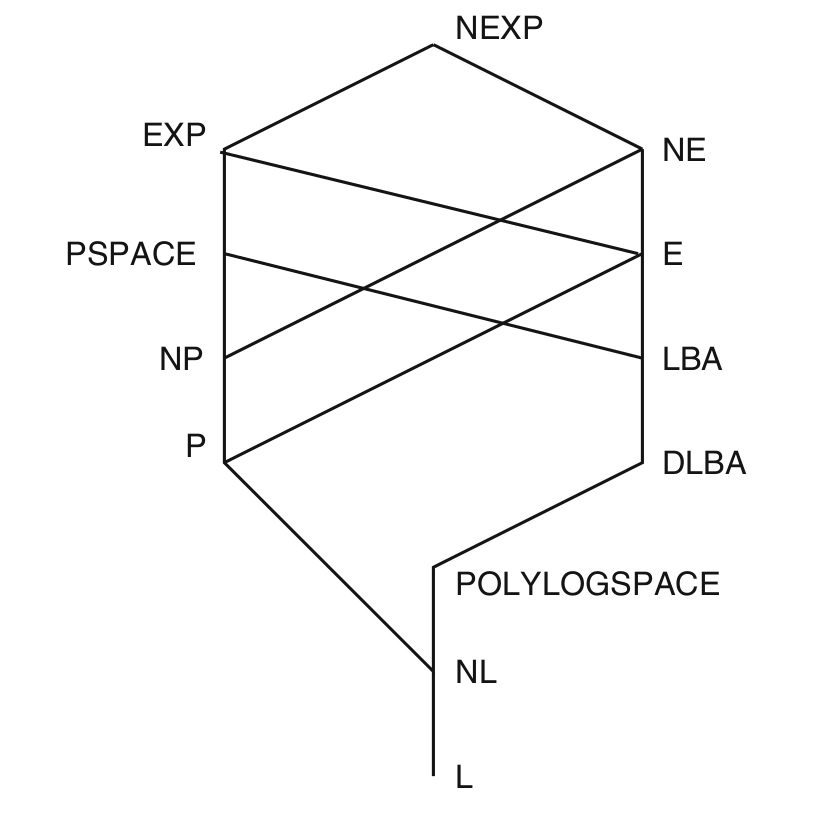
\includegraphics[width=0.38\textwidth]{hierarchy}
  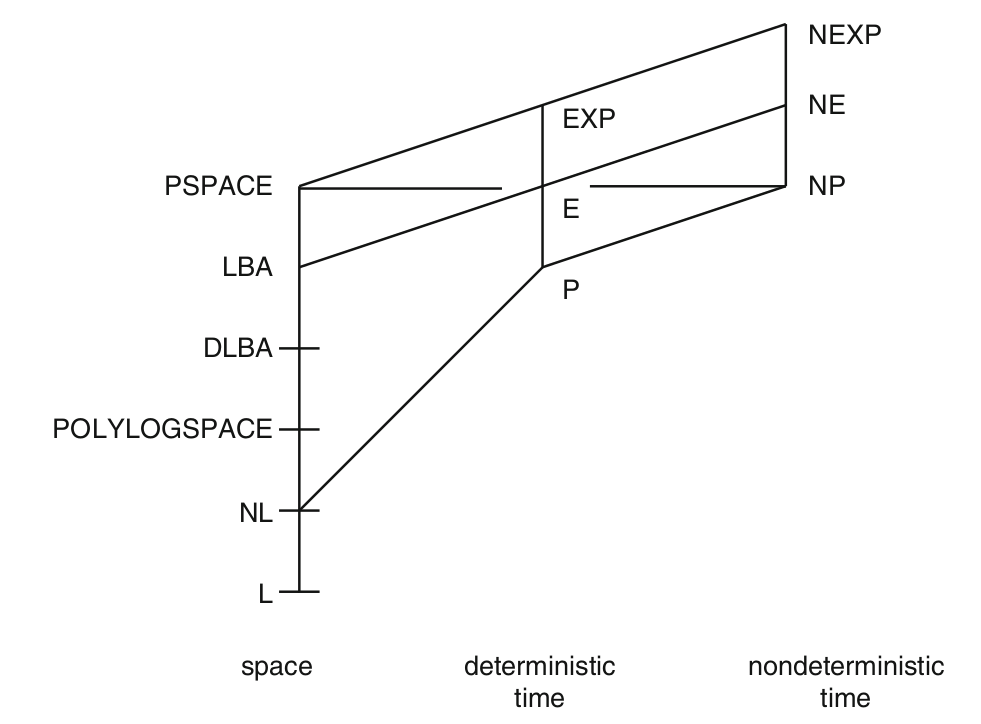
\includegraphics[width=0.6\textwidth]{hierarchy2}
\end{figure}

\key{Savitch (NSPACE($S(n)$) $\subseteq$ DSPACE($S^2(n)$))}
\begin{itemize}
  \item NL $\subseteq$ POLYLOGSPACE
  \item LBA $\subseteq$ PSPACE
\end{itemize}

\key{Space Hierarchy}
\begin{itemize}
  \item POLYLOGSPACE $\subseteq$ DLBA
\end{itemize}

\key{DSPACE($S(n)$) $\subseteq$ $\cup\{$DTIME($c^{S(n)})|c \ge 1\}$}
\begin{itemize}
  \item L $\subseteq$ P
  \item DLBA $\subseteq$ E
  \item PSPACE $\subseteq$ EXP
\end{itemize}

\key{NSPACE($S(n)$) $\subseteq$ $\cup\{$DTIME($c^{S(n)})|c \ge 1\}$.}
\begin{itemize}
  \item NL $\subseteq$ P 
  \item LBA $\subseteq$ E
\end{itemize}

\key{NTIME($S(n)$) $\subseteq$ DSPACE($S(n)$)}
\begin{itemize}
  \item NP $\subseteq$ PSPACE
\end{itemize}


\subsection{Separation Results}

\key{Theorem 5.15 (Space Hierarchy Theorem ).} Let $S(n)$ be fully space-
constructible. There is a language $L \in \text{DSPACE}(S(n))$ such that for every function
$S'(n)$, if $S'(n) \in o(S(n))$, then $L \notin \text{DSPACE}(S(n))$.

\key{Corollary 5.13.} $L \subset$ POLYLOGSPACE, POLYLOGSPACE $\subset$ DLBA, and DLBA
$\subset$ PSPACE.
\begin{align*}
\text{POLYLOGSPACE} &= \cup \{\text{DSPACE}((logn)^k ) | k \ge 1\}\\
&\subseteq \text{DSPACE}(n^\frac{1}{2})\\
&\subset \text{DLBA}.
\end{align*}

\key{Corollary 5.14.} LBA $\subset$ PSPACE.
\begin{align*}
\text{LBA} &= \text{NSPACE}(n), \text{by Corollary 5.1} \\
& \subseteq \text{DSPACE}(n^2 ), \text{by Theorem 5.13} \\
& \subset \text{DSPACE}(n^3 ), \text{by Theorem 5.15} \\
& \subseteq \text{PSPACE}.
\end{align*}

\key{Theorem 5.16 (Time Hierarchy Theorem).} Let $T$ be a fully time-constructible
function and assume that there exists a function $T'(n)$ so that
$T'(n)log(T'(n)) \in o(T(n))$.
Then there is a language $L \in \text{DTIME}(T(n))$ such that for every function 
$T'(n)$ such that $T'(n)log(T'(n)) \in o(T(n))$, $L \notin \text{DTIME}(T'(n))$.

\key{Corollary 5.15.} For every constant $c > 0$, DTIME($n^c$) $\subset$ DTIME($n^{c+1}$) and
DTIME($2^{cn}$) $\subset$ DTIME($2^{(c+1)n}$).

\key{Corollary 5.16.} P $\subset$ E and E $\subset$ EXP.

\subsection{Translation Techniques and Padding}

\key{Lemma 5.2.} Let $S(n)$ and $f(n)$ be fully space-constructible functions, where
$S(n) \ge n$ and $f(n) \ge n$. For a language $L$, define
$p(L) = \{x10^i | x \in L \text{ and }|x10^i | = f(|x|)\}$.
Then $L \in \text{NSPACE}(S(f(n))) \Leftrightarrow p(L) \in \text{NSPACE}(S(n))$.

\key{Theorem 5.17.} Let $S_1(n), S_2(n)$, and $f(n)$ be fully space-constructible functions,
where $S_1 (n) \ge n, S_2(n) \ge n$ and $f(n) \ge n$. Then
NSPACE($S_1(n)) \subseteq$ NSPACE($S_2(n)$) implies NSPACE($S_1(f(n)))
\subseteq$ NSPACE($S_2(f(n)))$.

\key{Example 5.5.} NSPACE($n^2$) $\subset$ NSPACE($n^3$).\\
Suppose for contradiction that NSPACE($n^3$) $\subseteq$ NSPACE($n^2$), then we 
have
\begin{align*}
  \text{NSPACE}(n^6) &\subseteq \text{NSPACE}(n^4) \text{ with } f(n)=n^2\\
  \text{NSPACE}(n^9) &\subseteq \text{NSPACE}(n^6) \text{ with } f(n)=n^3
\end{align*}
Then we have the following.
\begin{align*}
\text{NSPACE}(n^9) &\subseteq \text{NSPACE}(n^6) \\
&\subseteq \text{NSPACE}(n^4) \\
&\subseteq \text{DSPACE}(n^8), \text{ by Savitch theorem} \\
&\subset \text{DSPACE}(n^9), \text{by space hierarchy theorem} \\
&\subseteq \text{NSPACE}(n^9)
\end{align*}

\key{Example 5.6.} We use the analog of Theorem 5.17 for deterministic time to show
that DTIME($2^n$) $\subset$ DTIME($n2^n$).\\
Suppose for contradiction that DTIME($n2^n$) $\subseteq$ DTIME($2^n$), then we have 
\begin{align*}
\text{DTIME}(2^n2^{2^n}) &\subseteq \text{DTIME}(2^{2^n}) \text{ with } f(n) = 2^n\\
\text{DTIME}((n+2^n)2^{n+2^n}) &\subseteq \text{DTIME}(2^{n+2^n}) \text{ with }
f(n) = n+2^n\\
\text{DTIME}((n+2^n)2^{n}2^{2^n}) &\subseteq \text{DTIME}(2^{2^n}) \text{
combine above two.}
\end{align*}
Which violate the time hierarchy theorem.

\subsubsection{Tally Languages}

\key{Definition} For $L \in \Sigma^*$, let Tally(L) = $\{1^{n(w)} | w \in L\}$.

\key{Theorem 5.18.} NE $\subseteq$ E if and only if every tally language in NP belongs
to P.

\key{Corollary 5.17.} P = NP implies E = NE.

\section{Nondeterminism and NP-Completeness}

\subsection{Characterizing NP}

\key{Theorem 6.1.} A set $A$ belongs to NP if and only if there exist a polynomial
$p$ and a binary relation $R$ that is decidable in polynomial time such that for all words
in $\Sigma^*$,
$x \in A \Leftrightarrow \exists y [|y| \le p(|x|) \land R(x, y)]$.

\key{Verifier} Define a verifier for a language $A$ to be an algorithm $V$ such that
$A = \{x |\exists y[V \text{ accepts } \langle x, y \rangle ]\}$.

\key{Corollary 6.1.} NP is the class of all languages A having a polynomial-time
verifier.

\subsection{The Class P}

\subsection{Enumerations}

\key{Definition 6.1.} A class of sets $\mathscr{C}$ is effectively presentable if there is an
effective enumeration $\{M_i\}_i$ of Turing machines such that every Turing machine in the
enumeration halts on all inputs and $\mathscr{C} = \{L(M_i) | i \ge 0\}$.

\key{Theorem 6.2.} There is no effective enumeration of the class of all
deterministic Turing machines that operate in polynomial time. That is,
$S = \{i | \text{DM}_i \text{operates in polynomial time}\}$
is not a computably enumerable set.

\key{Theorem 6.3.} P and NP are effectively presentable:\\
NP = \{L(NP$_i) | i \ge 0\}$;\\
P = \{L(P$_i) | i \ge 0\}$;

\subsection{NP-Completeness}

\key{Definition 6.2.} A set $A$ is many-one reducible in polynomial time to a
set $B$
(notation: $A \le^P_m B$) if there exists a function $f$ that is computable
in polynomial time so that $x \in A \Leftrightarrow f(x) \in B$.

\key{Theorem 6.4.} NP $\ne$ E.

\key{Definition 6.3.} A set $A$ is $\le^P_m$-complete for NP (commonly
called NP-complete) if
\begin{enumerate}
  \item A $\in$ NP;
  \item for every set L $\in$ NP, L $\le^P_m$ A.
\end{enumerate}

\key{Theorem 6.5.} If $A$ is NP-complete, then $A \in P$ if and only if P =
NP.

\key{Universal set for NP} $\mathscr{U} = \{\langle i, x, 0^n \rangle |$ some
computation of NP$_i$ accepts $x$ in fewer than $n$ steps\}

\key{Theorem 6.6.} $\mathscr{U}$ is NP-complete.\\
For each $S\ in$ NP, there is some $i$ such
that $S = L(\text{NP}_i)$. Given $S = L(\text{NP}_i)$, define $f$ so that for
every word $x$, $f(x) = \langle i, x, 0^{p_i(|x|)} \rangle$. Then we have
\begin{align*}
  x \in S &\Leftrightarrow \text{NP}_i \text{accepts } x \\
  &\Leftrightarrow \text{NP}_i \text{accepts } x \text{ in } p_i(|x|) \text{ steps}\\
  &\Leftrightarrow \langle i, x, 0^{p_i(|x|)} \rangle \in \mathscr{U}\\
  &\Leftrightarrow f(x) \in \mathscr{U}
\end{align*}

\subsection{The Cook-Levin Theorem}

\key{Theorem 6.7.} SAT belongs to NP.

\key{Theorem 6.8.} CNF-SAT is an NP-complete problem.

\subsection{More NP-Complete Problems}

\key{Proposition 6.1.} If A is NP-complete, $A \le_m^P B$, and $B \in$ NP, then B is NP-complete.

\key{Corollary 6.2.} SAT is NP-complete.

\subsubsection{The Diagonal Set Is NP-Complete}

\key{$K$} $K = \{i | \text{NP}_i \text{ accepts } i \text{ within } |i| \text{
steps}\}$.

\subsubsection{Some Natural NP-Complete Problems}

\key{Theorem 6.10.} 3SAT is NP-complete.

\key{Vertex cover} A vertex cover of a graph $G = (V, E)$ is a subset $V'$ of
$V$ that, for each edge $(u, v) \in E$, contains at least one of the
adjacent vertices $u$ and $v$.

\key{VERTEX COVER}\\
\textbf{instance} A graph $G = (V, E)$ and a positive integer $k \le ||V||$ .\\
\textbf{question} Is there a vertex cover of size $\le k$ for $G$?

\key{Theorem 6.11.} VERTEX COVER is NP-complete.

\key{Clique} A complete subgraph of G

\key{CLIQUE} \\
\textbf{instance} A graph $G = (V, E)$ and a positive integer $j \le ||V||$ .\\
\textbf{question} Does $G$ contain a clique of size $j$ or more?

\key{Theorem 6.12.} CLIQUE is NP-complete.

\section{Relative Computability}

\key{$L(M,A)$} The language accepted by $M$ with oracle $A$ is denoted $L(M, A)$

\key{Definition 7.1.} A set $A$ is Turing-reducible to $B$ in polynomial-time 
($A \le_T^P B$) if there exists a deterministic polynomial-time-bounded oracle 
Turing machine M such that $A = L(M, B)$.

\key{Theorem 7.1.} There is a decidable set $A$ such that $\overline{A} \le_m^P A$ (and
$A \ne \Sigma^*$ and $A \ne \emptyset$).

\subsection{NP-Hardness}

\key{Definition 7.2.} A set $A$ is NP-hard if, for every $L \in$ NP,
$L \le^P_T A$.
\begin{itemize}
  \item An NP-hard set does not need to belong to NP
  \item We use Turing reducibility this time instead of many-one reducibility
  \item Every NP-complete set is NP-hard
  \item The complement of every NP-complete set is NP-hard
\end{itemize}

\key{Proposition 7.1.} If $A$ is NP-hard and $A \in $P, then NP = P.

\key{Theorem 7.3}. For each decidable set $A \notin $ P, there is a
decidable set $B$ such that $A \le^P_T B$ but $A \nleq^P_m B$. In particular, 
$A \le^P_T B$ by a reduction procedure that on every input makes two queries to the oracle.

\key{Corollary 7.1.} If P $\ne$ NP, then there exists a set that is $\le^P_T$-hard 
for NP but not $\le^P_m$-hard for NP.

\key{Theorem 7.4.} If A is $\le^P_T$-complete for NP, then $A \in P$ if and only if P = NP.

\subsection{Search Problems}

\key{Definition 7.3.} Let $L \in NP$ and let $R_L$ and $p_L$ define $L$.
Prefix($R_L, p_L$) = $\{\langle x, u \rangle | u$ is a prefix of a witness $y$ such that
$|y| \le p_L(|x|)$ and $R_L(x, y)$\}.

\key{Proposition 7.2.}
\begin{enumerate}
  \item Prefix($R_L,p_ L) \in$ NP.
  \item $L \le^P_m$ Prefix($R_L,p_ L$).
  \item If $L$ is NP-complete, then Prefix($R_L,p_L$) is NP-complete.
  \item If $L$ is $\le^P_T$-complete for NP, then Prefix($R_L,p_ L$) is
    $\le^P_T$-complete for NP.
\end{enumerate}

\key{Theorem 7.5.} The search problem for $R_L$ and $p_L$ is Turing-reducible in
polynomial time to Prefix($R_L,p_L$).

\subsection{The Structure of NP}

\key{Definition 7.6.} Two sets $A$ and $B$ are equal almost everywhere ($A = B$ a.e.)
if the symmetric difference of $A$ and $B$, $A \vartriangle B$, is a finite set.
A class of sets $\mathscr{C}$ is closed under finite variations if $A \in
\mathscr{C}$ and $A = B$ a.e. implies $B \in \mathscr{C}$.

The complexity classes P and NP are closed under finite variation.

\key{Fast function} Define a function $f : N \rightarrow N$ to be fast if
the following two properties hold:
\begin{enumerate}
  \item For all $n \in N$, $f(n) > n$, and
  \item There is a Turing machine $M$ that computes $f$ in unary notation such
    that $M$ writes a symbol on its output tape every move of its computation. In particular,
    for every $n$, $f(n) = T_M(n)$.
\end{enumerate}

\key{Proposition 7.3.} For every total computable function $f$ , there is a fast
function $f'$ such that, for all $n$, $f'(n) > f(n)$.

\key{$\mathbf{G[f]}$} $G[f] = \{ x \in \Sigma^* | f^n(0) \le |x| < f^{n+1}(0)$, for even
$n$\}.

\key{Lemma 7.1.} If $f$ is fast, then $G[f] \in P$.


\key{Theorem 7.6.} Let $A$ and $B$ be decidable sets and let $\mathscr{C}_1$ and
$\mathscr{C}_2$ be classes of decidable sets with the following properties:
\begin{enumerate}
  \item $A \notin \mathscr{C}_1$ and $B \notin \mathscr{C}_2$;
  \item $\mathscr{C}_1$ and $\mathscr{C}_2$ are effectively presentable; and
  \item $\mathscr{C}_1$ and $\mathscr{C}_2$ are closed under finite variations.
\end{enumerate}
Then there exists a decidable set C such that
\begin{enumerate}
  \item $C \notin \mathscr{C}_1$ and $C \notin \mathscr{C}_2$, and
  \item If $A \in$ P and $B \ne \emptyset$ and $B \ne \Sigma^*$, then $C
    \le^P_m B$.
\end{enumerate}

\key{Lemma 7.2.} The class of all $\le^P_T$-complete sets for NP is effectively presentable.

\key{Corollary 7.4.} If P $\ne$ NP, then there exists a set $C$ in NP-P
that is not $\le^P_T$-complete for NP.\\
Let $A=\emptyset$, $B=$SAT, and let $\mathscr{C}_1$ be collection of all
$\le^P_T$-complete sets of NP, and $\mathscr{C}_2 =$P.
\begin{enumerate}
  \item $C \notin$ P and $C$ is not $\le^P_T$-complete for NP
  \item $C \le^P_m$ SAT, so $C \in$ NP.
\end{enumerate}

\key{$\mathbf{X \oplus Y}$} $X \oplus Y = \{0x | x \in X\} \bigcup \{1x | x \in
Y\}$.

\key{Corollary 7.5.} If P $\ne$ NP, then there exist $\le^P_T$-incomparable
members of NP. That is, there exist sets $C_0$ and $C_1$ in NP such that 
$C_0 \nleq^P_T C_1$ and $C_1 \nleq^P_T C_0$ .

\key{Corollary 7.6.} If P $\ne$ NP, then for every set $B \in$ NP-P, there is a 
set $C \in$ NP-P such that $C \le^P_T B$ and $B \nleq^P_T C$.\\
If P $\ne$ NP, then NP contains countably many distinct $\le^P_T$-degrees that form 
an infinite descending hierarchy.

\key{Corollary 7.7.} If P = NP, then NP$-$P is not effectively presentable.

\subsubsection{Composite Number and Graph Isomorphism}


\subsection{The Polynomial Hierarchy}

For any set $A$, let P$^A = \{B | B \le^P_T A\}$ and let NP$^A = \{B |
B\le^{NP}_T A\}$. So P$^A$(NP$^A$) is the class of sets accepted deterministically
(nondeterministically, respectively) in polynomial time relative to the set $A$.

\key{Polynomial hierarchy} $\Sigma^P_0 = \Pi^P_0 = \Delta^P_0 =$ P
\begin{align*}
  \Sigma^P_{k+1} & = \text{NP}^{\Sigma^P_{k}} \\
  \Pi^P_{k+1} &= \text{co-}\Sigma^P_{k+1} \\
  \Delta^P_{k+1} &= \text{P}^{\Sigma^P_{k}} 
\end{align*}

\key{Proposition 7.4.} For all $k \ge 0$, $\Sigma_k^P \bigcup \Pi_k^P \subseteq
\Delta_{k+1}^P \subseteq \Sigma_{k+1}^P \bigcap \Pi_{k+1}^P$.

\key{Proposition 7.5.} PH $\subseteq$ PSPACE, where PH= $\bigcup \{\Sigma^P_k|k \ge
0\}$.

\key{Theorem 7.10.} If for some $k \ge 1, \Sigma_k^ P = \Pi_k^P$ , then for all
$j \ge k$, $\Sigma^P_j = \Pi^P_j = \Sigma_k^P$ .

\key{Corollary 7.8.} $A \le^P_m B$ and $B \in \Sigma�_n^P$ implies $A \in
\Sigma_n^P$.


\end{document}
